\documentclass[11pt, a4paper]{article}

% Fonts and Encoding
\usepackage[utf8]{inputenc}
\usepackage[T1]{fontenc}
\usepackage{lmodern}
% Math and Symbols
\usepackage{amsmath, amssymb, amsthm, amsfonts, mathrsfs, mathtools}

% Layout and Geometry
\usepackage{geometry}
\geometry{a4paper, margin=1in}

% Formatting and Graphics
\usepackage{graphicx, xcolor, enumitem, booktabs, array, tabularx}

% TikZ for Illustrations
\usepackage{tikz}
\usetikzlibrary{arrows.meta, positioning, shapes.geometric, calc, backgrounds, matrix}

% Clickable Links and TOC
\usepackage{hyperref}
\hypersetup{
    colorlinks=true,
    linkcolor=blue,
    filecolor=magenta,      
    urlcolor=cyan,
    pdftitle={Advanced Mathematics Topic},
}

% Theorem Environments
\newtheorem{theorem}{Theorem}[section]
\newtheorem{lemma}[theorem]{Lemma}
\newtheorem{proposition}[theorem]{Proposition}
\newtheorem{corollary}[theorem]{Corollary}
\theoremstyle{definition}
\newtheorem{definition}{Definition}[section]
\newtheorem{axiom}{Axiom}[section]
\newtheorem{example}{Example}[section]
\theoremstyle{remark}
\newtheorem{remark}{Remark}[section]

% Custom Commands (Enforced standard notation)
\newcommand{\R}{\mathbb{R}}
\newcommand{\N}{\mathbb{N}}
\newcommand{\Z}{\mathbb{Z}}
\newcommand{\Q}{\mathbb{Q}}
\newcommand{\E}{\mathbb{E}}
\newcommand{\Prob}{\mathbb{P}}
\newcommand{\F}{\mathcal{F}}

\title{\textbf{Mastery Guide: Laplace Transforms (Section 7.2)}}
\author{Tashfeen mran}
\date{\today}

\begin{document}

\maketitle
\tableofcontents
\newpage

\section{Part 1: Comprehensive Introduction, Context, and Prerequisites}

\subsection{Core Concepts}
The \textbf{Laplace Transform} is a powerful integral transform used to switch a function from the \textit{time domain} (where the independent variable is typically $t$, representing time) to the \textit{frequency domain} (where the independent variable is $s$, a complex frequency parameter). 

Mathematically, the Laplace transform of a function $f(t)$ defined for $t \ge 0$ is denoted by $\mathscr{L}\{f(t)\}$ or $F(s)$, and is defined by the improper integral:
\[
F(s) = \int_{0}^{\infty} e^{-st} f(t) \, dt
\]
This transformation is a \textit{linear operator}, meaning it distributes over addition and scalar multiplication. By transforming differential equations into algebraic equations in terms of $s$, the Laplace transform drastically simplifies the process of solving Initial Value Problems (IVPs).

\subsection{Intuition and Derivation}
Why multiply by $e^{-st}$ and integrate to infinity? The term $e^{-st}$ acts as a \textit{damping factor}. Many functions, like $e^{2t}$ or $t^3$, grow infinitely large as $t \to \infty$. By multiplying by a decaying exponential $e^{-st}$ (where $s$ is chosen to be large enough), we force the overall product to decay to zero, ensuring the improper integral converges to a finite area. The resulting area depends entirely on the parameter $s$, hence yielding a new function $F(s)$.

\subsection{Historical Context and Motivation}
The technique is named after the French mathematician Pierre-Simon Laplace, who used similar transformations in his work on probability theory in the late 18th century. However, it was the English electrical engineer Oliver Heaviside who, in the late 19th century, popularized operational calculus to solve complex differential equations in electrical circuits. Heaviside's methods were initially criticized for lacking mathematical rigor, but mathematicians later proved that his operational techniques were perfectly justified by the Laplace transform. Today, it is the bedrock of control theory, signal processing, and systems engineering.

\subsection{Key Formulas}
\begin{itemize}
    \item \textbf{Definition:} $\mathscr{L}\{f(t)\} = \int_{0}^{\infty} e^{-st} f(t) \, dt$
    \item \textbf{Linearity:} $\mathscr{L}\{a f(t) + b g(t)\} = a \mathscr{L}\{f(t)\} + b \mathscr{L}\{g(t)\}$
    \item \textbf{First Translation (Shift) Theorem:} $\mathscr{L}\{e^{at} f(t)\} = F(s - a)$
\end{itemize}

\subsection{Prerequisites}
To master this topic, you must be proficient in:
\begin{enumerate}
    \item \textbf{Improper Integrals:} Evaluating limits as the upper bound of an integral approaches infinity.
    \item \textbf{Integration by Parts:} Specifically, the tabular method for repeated integration.
    \item \textbf{Algebraic Manipulation:} Completing the square and partial fraction decomposition.
    \item \textbf{Limits and Continuity:} Understanding left-hand limits, right-hand limits, and jump discontinuities.
\end{enumerate}

\newpage
\section{Part 2: Detailed Homework Solutions}

\subsection{Problem 1}
\textbf{Statement:} Let $f(t)$ be a function on $[0, \infty)$. The Laplace transform of $f$ is the function $F$ defined by the integral $F(s) = \int_{0}^{\infty} e^{-st} f(t) \, dt$. Use this definition to determine the Laplace transform of $f(t) = 7t^3$.

\textbf{Solution:}
We set up the improper integral according to the definition:
\[
F(s) = \int_{0}^{\infty} e^{-st} (7t^3) \, dt = 7 \int_{0}^{\infty} t^3 e^{-st} \, dt
\]
To integrate $t^3 e^{-st}$, we use integration by parts repeatedly (tabular method). 
Let $u = t^3$ (differentiate to $0$) and $dv = e^{-st} \, dt$ (integrate repeatedly):
\renewcommand{\arraystretch}{1.5}
\begin{center}
\begin{tabularx}{0.6\textwidth}{>{\centering\arraybackslash}X >{\centering\arraybackslash}X >{\centering\arraybackslash}X}
\toprule
\textbf{Sign} & \textbf{Differentiate ($u$)} & \textbf{Integrate ($dv$)} \\
\midrule
$+$ & $t^3$ & $e^{-st}$ \\
$-$ & $3t^2$ & $-\frac{1}{s} e^{-st}$ \\
$+$ & $6t$ & $\frac{1}{s^2} e^{-st}$ \\
$-$ & $6$ & $-\frac{1}{s^3} e^{-st}$ \\
$+$ & $0$ & $\frac{1}{s^4} e^{-st}$ \\
\bottomrule
\end{tabularx}
\end{center}

Multiplying diagonally and applying the signs, the antiderivative is:
\[
\int t^3 e^{-st} \, dt = -e^{-st} \left( \frac{t^3}{s} + \frac{3t^2}{s^2} + \frac{6t}{s^3} + \frac{6}{s^4} \right)
\]
Now, we evaluate this from $0$ to $\infty$:
\[
F(s) = 7 \lim_{R \to \infty} \left[ -e^{-st} \left( \frac{t^3}{s} + \frac{3t^2}{s^2} + \frac{6t}{s^3} + \frac{6}{s^4} \right) \right]_{0}^{R}
\]
For $s > 0$, as $R \to \infty$, the exponential decay $e^{-sR}$ dominates the polynomial terms, so the upper limit evaluates to $0$. 
At the lower limit $t = 0$, all terms containing $t$ vanish, leaving only the constant term:
\[
F(s) = 7 \left( 0 - \left( -e^{0} \left( 0 + 0 + 0 + \frac{6}{s^4} \right) \right) \right) = 7 \left( \frac{6}{s^4} \right) = \frac{42}{s^4}
\]
\textbf{Final Answer:} $F(s) = \frac{42}{s^4}$. It is defined for $s > 0$.

\vspace{1em}
\subsection{Problem 2}
\textbf{Statement:} Determine whether $f(t)$ is continuous, piecewise continuous, or neither on $[0,10]$, and sketch the graph of $f(t)$.
\[
f(t) = 
\begin{cases} 
40, & 0 \le t < 3 \\ 
t + 8, & 3 < t < 6 \\ 
(t - 3)^2 + 20, & 6 < t \le 10 
\end{cases}
\]

\textbf{Solution:}
A function is piecewise continuous on a finite interval if it is continuous everywhere except at a finite number of points, and at those points, it has finite jump discontinuities (both left and right limits exist and are finite).

Let's check the boundaries at $t = 3$ and $t = 6$:
\begin{itemize}
    \item \textbf{At $t = 3$:} 
    \[ \lim_{t \to 3^-} f(t) = 40 \quad \text{and} \quad \lim_{t \to 3^+} f(t) = 3 + 8 = 11 \]
    Since $40 \neq 11$, there is a finite jump discontinuity at $t = 3$.
    \item \textbf{At $t = 6$:}
    \[ \lim_{t \to 6^-} f(t) = 6 + 8 = 14 \quad \text{and} \quad \lim_{t \to 6^+} f(t) = (6 - 3)^2 + 20 = 9 + 20 = 29 \]
    Since $14 \neq 29$, there is a finite jump discontinuity at $t = 6$.
\end{itemize}
Because all discontinuities are finite jumps, the function is \textbf{piecewise continuous}.

\textbf{Graph Sketch:}
\begin{center}
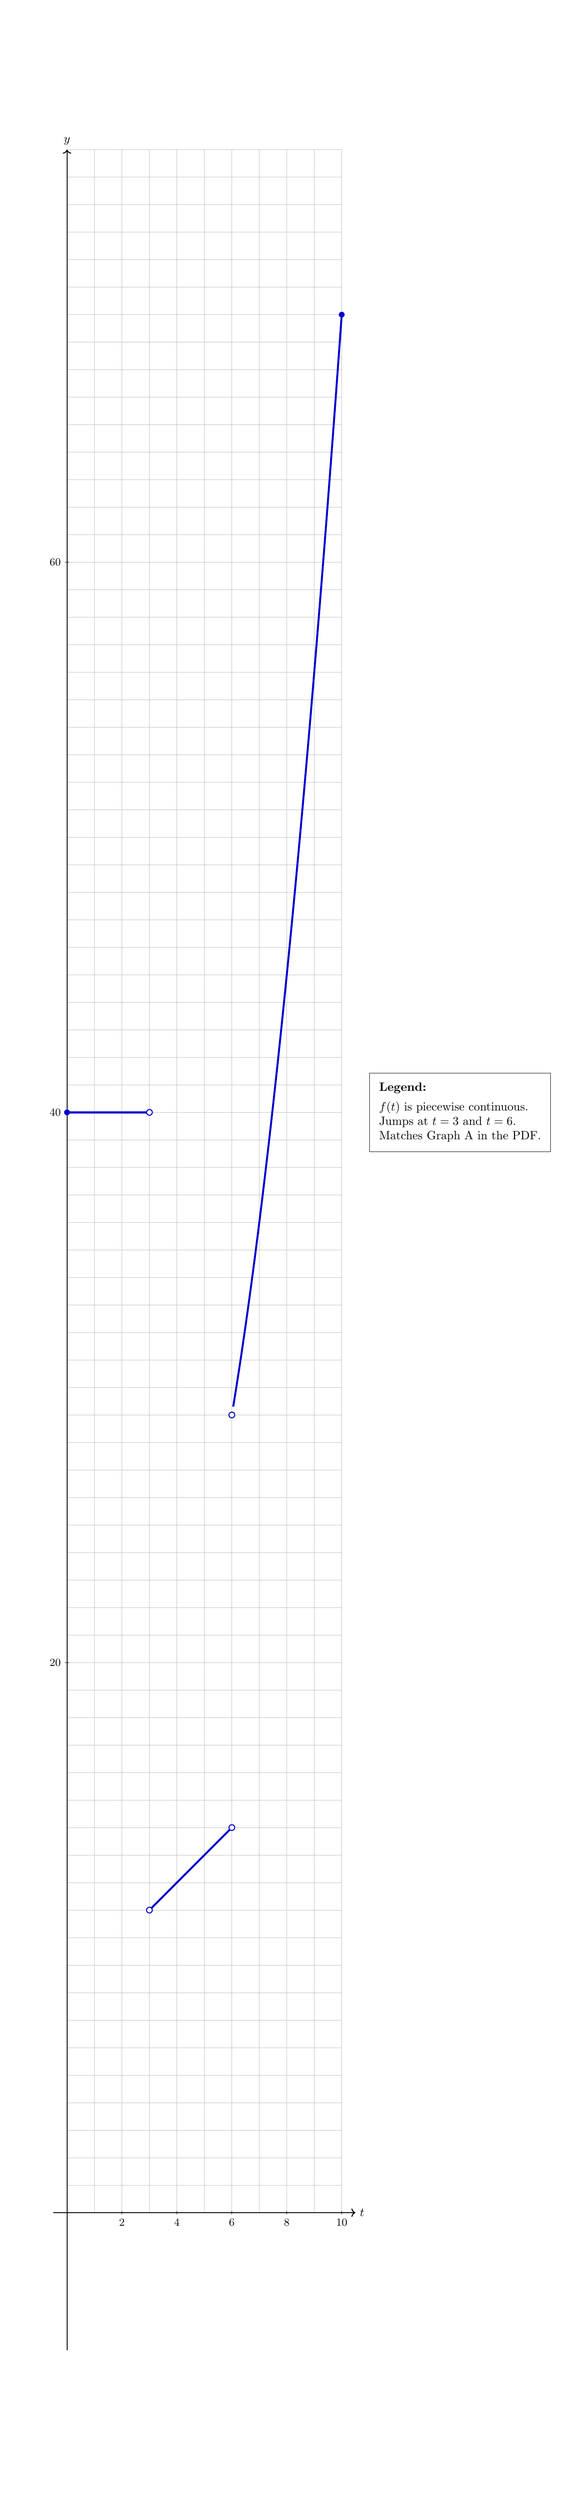
\begin{tikzpicture}[scale=0.8]
    \fill[white] (-2,-10) rectangle (14, 80);
    \draw[lightgray, very thin, step=1] (0,0) grid (10,75);
    \draw[->, thick] (-0.5,0) -- (10.5,0) node[right] {$t$};
    \draw[->, thick] (0,-5) -- (0,75) node[above] {$y$};
    
    % Ticks
    \foreach \x in {2,4,6,8,10} \draw (\x, 2pt) -- (\x, -2pt) node[below] {\small $\x$};
    \foreach \y in {20,40,60} \draw (2pt, \y) -- (-2pt, \y) node[left] {\small $\y$};

    % 0 to 3: y=40
    \draw[ultra thick, blue!80!black] (0,40) -- (2.95,40);
    \fill[blue!80!black] (0,40) circle (3pt);
    \draw[blue!80!black, fill=white, thick] (3,40) circle (3pt);

    % 3 to 6: y=t+8
    \draw[ultra thick, blue!80!black] (3.05,11.05) -- (5.95,13.95);
    \draw[blue!80!black, fill=white, thick] (3,11) circle (3pt);
    \draw[blue!80!black, fill=white, thick] (6,14) circle (3pt);

    % 6 to 10: y=(t-3)^2+20
    \draw[ultra thick, blue!80!black, domain=6.05:10, samples=50] plot (\x, {(\x-3)^2+20});
    \draw[blue!80!black, fill=white, thick] (6,29) circle (3pt);
    \fill[blue!80!black] (10,69) circle (3pt);

    % Legend
    \node[align=left, anchor=west, inner sep=8pt, draw, fill=white] at (11, 40) {
        \textbf{Legend:} \\[4pt]
        $f(t)$ is piecewise continuous. \\
        Jumps at $t=3$ and $t=6$. \\
        Matches Graph A in the PDF.
    };
\end{tikzpicture}
\end{center}
\textbf{Final Answer:} A. piecewise continuous. The correct graph is A.

\vspace{1em}
\subsection{Problem 3}
\textbf{Statement:} Determine the Laplace transform of $f(t) = t e^{-6t}$.

\textbf{Solution:}
We use the First Translation (Shift) Theorem, which states that $\mathscr{L}\{e^{at} f(t)\} = F(s - a)$, where $F(s) = \mathscr{L}\{f(t)\}$.
Here, our base function is $f(t) = t$, and our exponential shift is $a = -6$.
1. Find the transform of the base function:
\[
\mathscr{L}\{t\} = \frac{1}{s^2}, \quad s > 0
\]
2. Apply the shift $s \to s - (-6) = s + 6$:
\[
\mathscr{L}\{t e^{-6t}\} = \frac{1}{(s + 6)^2}
\]
The restriction shifts from $s > 0$ to $s + 6 > 0 \implies s > -6$.

\textbf{Final Answer:} $F(s) = \frac{1}{(s+6)^2}$. It is defined for $s > -6$.

\vspace{1em}
\subsection{Problem 4}
\textbf{Statement:} Determine the Laplace transform of $f(t) = \cos bt$, where $b$ is a constant.

\textbf{Solution:}
Using the standard Laplace transform table provided in the assignment:
\[
\mathscr{L}\{\cos bt\} = \frac{s}{s^2 + b^2}
\]
Because the function does not contain an exponential growth factor, the integral converges as long as the damping factor $e^{-st}$ decays, which requires $s > 0$.

\textbf{Final Answer:} $F(s) = \frac{s}{s^2 + b^2}$. It is defined for $s > 0$.

\vspace{1em}
\subsection{Problem 5}
\textbf{Statement:} Determine the Laplace transform of $f(t) = e^{-t} \sin 5t$.

\textbf{Solution:}
We again apply the First Translation Theorem. 
1. The base function is $\sin 5t$. From the table:
\[
\mathscr{L}\{\sin 5t\} = \frac{5}{s^2 + 5^2} = \frac{5}{s^2 + 25}, \quad s > 0
\]
2. The exponential factor is $e^{-t}$, meaning $a = -1$. We shift $s \to s - (-1) = s + 1$:
\[
\mathscr{L}\{e^{-t} \sin 5t\} = \frac{5}{(s + 1)^2 + 25}
\]
The domain restriction shifts from $s > 0$ to $s + 1 > 0 \implies s > -1$.

\textbf{Final Answer:} $F(s) = \frac{5}{(s+1)^2 + 25}$. It is defined for $s > -1$.

\vspace{1em}
\subsection{Problem 6}
\textbf{Statement:} Use the Laplace transform table and linearity to determine $\mathscr{L}\{3e^{-6t} - t^3 + t - 6\}$.

\textbf{Solution:}
By the linearity of the Laplace transform:
\[
\mathscr{L}\{3e^{-6t} - t^3 + t - 6\} = 3\mathscr{L}\{e^{-6t}\} - \mathscr{L}\{t^3\} + \mathscr{L}\{t\} - 6\mathscr{L}\{1\}
\]
We evaluate each term using the table:
\begin{align*}
    3\mathscr{L}\{e^{-6t}\} &= 3 \left( \frac{1}{s + 6} \right) = \frac{3}{s + 6}, \quad s > -6 \\ [4pt]
    -\mathscr{L}\{t^3\} &= -\frac{3!}{s^4} = -\frac{6}{s^4}, \quad s > 0 \\ [4pt]
    \mathscr{L}\{t\} &= \frac{1}{s^2}, \quad s > 0 \\ [4pt]
    -6\mathscr{L}\{1\} &= -6 \left( \frac{1}{s} \right) = -\frac{6}{s}, \quad s > 0
\end{align*}
Combining them yields:
\[
F(s) = \frac{3}{s + 6} - \frac{6}{s^4} + \frac{1}{s^2} - \frac{6}{s}
\]
The overall restriction on $s$ is the most restrictive condition among all individual terms. We need $s > -6$ AND $s > 0$. The intersection of these intervals is $s > 0$.

\textbf{Final Answer:} $F(s) = \frac{3}{s + 6} - \frac{6}{s^4} + \frac{1}{s^2} - \frac{6}{s}$. The restriction is $s > 0$.

\vspace{1em}
\subsection{Problem 7}
\textbf{Statement:} Determine $\mathscr{L}\{e^{3t} \sin 6t - t^2 + e^{2t}\}$.

\textbf{Solution:}
Apply linearity:
\[
\mathscr{L}\{e^{3t} \sin 6t\} - \mathscr{L}\{t^2\} + \mathscr{L}\{e^{2t}\}
\]
Evaluate each term:
\begin{align*}
    \mathscr{L}\{e^{3t} \sin 6t\} &= \frac{6}{(s - 3)^2 + 36}, \quad s > 3 \\ [4pt]
    -\mathscr{L}\{t^2\} &= -\frac{2!}{s^3} = -\frac{2}{s^3}, \quad s > 0 \\ [4pt]
    \mathscr{L}\{e^{2t}\} &= \frac{1}{s - 2}, \quad s > 2
\end{align*}
Combining them:
\[
F(s) = \frac{6}{(s - 3)^2 + 36} - \frac{2}{s^3} + \frac{1}{s - 2}
\]
The restrictions are $s > 3$, $s > 0$, and $s > 2$. The most restrictive condition is $s > 3$.

\textbf{Final Answer:} $F(s) = \frac{6}{(s - 3)^2 + 36} - \frac{2}{s^3} + \frac{1}{s - 2}$. The restriction is $s > 3$.

\vspace{1em}
\subsection{Problem 8}
\textbf{Statement:} Determine $\mathscr{L}\{2t^2 e^{-3t} - e^{8t} \cos \sqrt{6}t\}$.

\textbf{Solution:}
Apply linearity:
\[
2\mathscr{L}\{t^2 e^{-3t}\} - \mathscr{L}\{e^{8t} \cos \sqrt{6}t\}
\]
Evaluate the first term using the shift theorem ($a = -3$) on $t^2$:
\[
2 \left( \frac{2!}{(s - (-3))^3} \right) = \frac{4}{(s + 3)^3}, \quad s > -3
\]
Evaluate the second term using the shift theorem ($a = 8$) on $\cos \sqrt{6}t$:
\[
\frac{s - 8}{(s - 8)^2 + (\sqrt{6})^2} = \frac{s - 8}{(s - 8)^2 + 6}, \quad s > 8
\]
Combining them:
\[
F(s) = \frac{4}{(s + 3)^3} - \frac{s - 8}{(s - 8)^2 + 6}
\]
The restrictions are $s > -3$ and $s > 8$. The intersection is $s > 8$.

\textbf{Final Answer:} $F(s) = \frac{4}{(s + 3)^3} - \frac{s - 8}{(s - 8)^2 + 6}$. The restriction is $s > 8$.

\vspace{1em}
\subsection{Problem 9}
\textbf{Statement:} Determine whether $f(t)$ is continuous, piecewise continuous, or neither on $[0,10]$, and sketch the graph.
\[
f(t) = 
\begin{cases} 
\frac{\sin t}{t}, & t \neq 0 \\ 
0, & t = 0 
\end{cases}
\]

\textbf{Solution:}
First, we analyze the behavior at $t = 0$. The limit of the function as $t \to 0$ is a well-known fundamental trigonometric limit:
\[
\lim_{t \to 0} \frac{\sin t}{t} = 1
\]
However, the function is explicitly defined as $f(0) = 0$. Since the limit exists and is finite ($1$), but does not equal the function value ($0$), there is a \textit{removable discontinuity} at $t = 0$. 
Because the discontinuity is finite, the function satisfies the definition of being \textbf{piecewise continuous}.

\textbf{Graph Sketch:}
\begin{center}
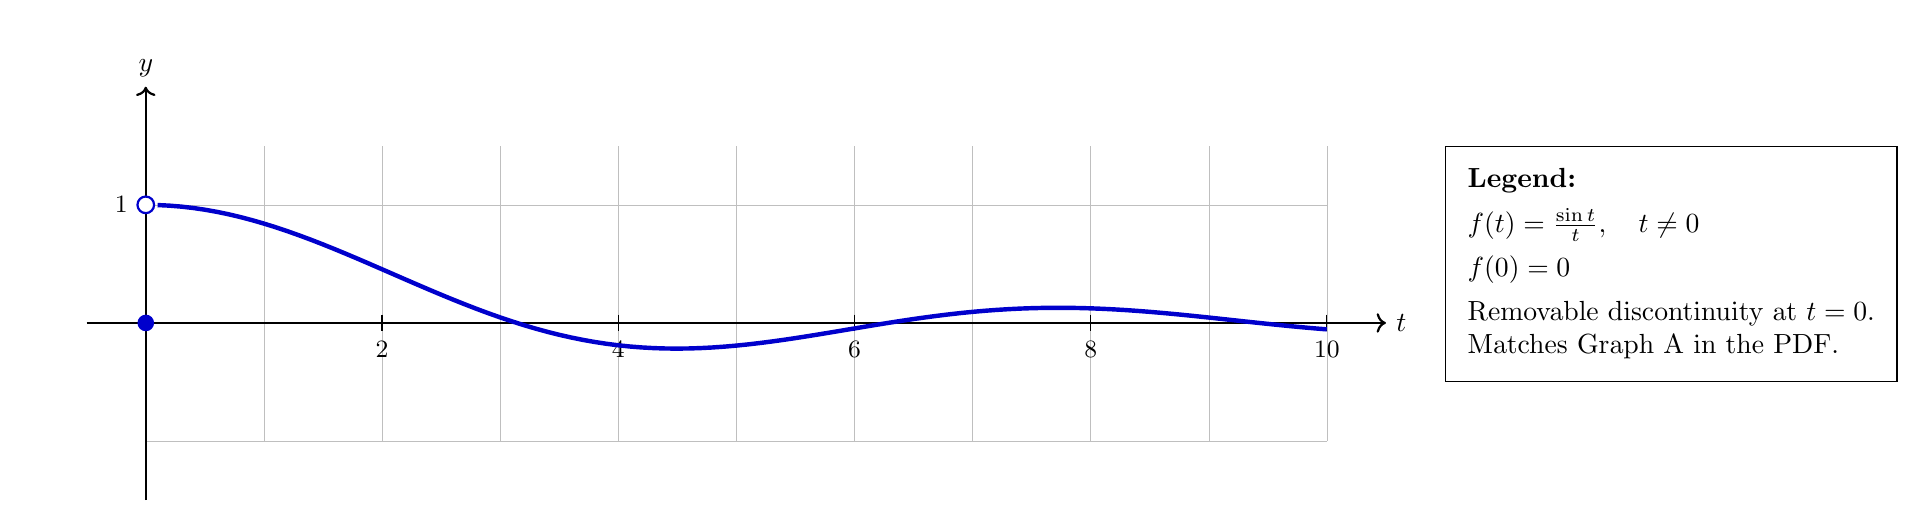
\begin{tikzpicture}[scale=1.5]
    \fill[white] (-1,-1.5) rectangle (11, 2.5);
    \draw[lightgray, very thin, step=1] (0,-1) grid (10,1.5);
    \draw[->, thick] (-0.5,0) -- (10.5,0) node[right] {$t$};
    \draw[->, thick] (0,-1.5) -- (0,2) node[above] {$y$};
    
    % Ticks
    \foreach \x in {2,4,6,8,10} \draw (\x, 2pt) -- (\x, -2pt) node[below] {\small $\x$};
    \draw (2pt, 1) -- (-2pt, 1) node[left] {\small $1$};

    % sin(t)/t curve
    \draw[ultra thick, blue!80!black, domain=0.1:10, samples=100] plot (\x, {sin(\x r)/\x});
    
    % Hole at (0,1)
    \draw[blue!80!black, fill=white, thick] (0,1) circle (2pt);
    
    % Solid dot at (0,0)
    \fill[blue!80!black] (0,0) circle (2pt);

    % Legend
    \node[align=left, anchor=west, inner sep=8pt, draw, fill=white] at (11, 0.5) {
        \textbf{Legend:} \\[4pt]
        $f(t) = \frac{\sin t}{t}, \quad t \neq 0$ \\[4pt]
        $f(0) = 0$ \\[4pt]
        Removable discontinuity at $t=0$. \\
        Matches Graph A in the PDF.
    };
\end{tikzpicture}
\end{center}
\textbf{Final Answer:} A. piecewise continuous. The correct graph is A.

\vspace{1em}
\subsection{Problem 10}
\textbf{Statement:} Which of the following functions are of exponential order? Select all that apply.

\textbf{Solution:}
A function $f(t)$ is of \textit{exponential order} if there exist constants $M > 0$, $c$, and $T > 0$ such that $|f(t)| \le M e^{ct}$ for all $t > T$. Essentially, the function cannot grow faster than an exponential function as $t \to \infty$.

Let's evaluate each option:
\renewcommand{\arraystretch}{1.5}
\begin{center}
\begin{tabularx}{\textwidth}{>{\hsize=0.1\hsize}X >{\hsize=0.3\hsize}X >{\hsize=0.6\hsize}X}
\toprule
\textbf{Opt} & \textbf{Function} & \textbf{Analysis} \\
\midrule
A & $4 - e^{t^2} + \cos 5t$ & \textbf{No.} The term $e^{t^2}$ grows faster than $e^{ct}$ for any constant $c$. \\
\addlinespace[4pt]
B & $\frac{1}{t^2+1}$ & \textbf{Yes.} This function is bounded by $1$. Any bounded function is of exponential order (choose $c=0, M=1$). \\
\addlinespace[4pt]
C & $t \ln t$ & \textbf{Yes.} Polynomial and logarithmic growth is strictly slower than exponential growth. \\
\addlinespace[4pt]
D & $e^{\frac{t^2}{t+5}}$ & \textbf{Yes.} By polynomial division, $\frac{t^2}{t+5} = t - 5 + \frac{25}{t+5}$. For large $t$, this behaves like $t$. Thus, $e^{\frac{t^2}{t+5}} \le e^t$. \\
\addlinespace[4pt]
E & $100 e^{50t}$ & \textbf{Yes.} This is exactly in the form $M e^{ct}$ with $M=100, c=50$. \\
\addlinespace[4pt]
F & $\cosh(t^2)$ & \textbf{No.} $\cosh(t^2) = \frac{e^{t^2} + e^{-t^2}}{2}$, which contains the hyper-exponential term $e^{t^2}$. \\
\addlinespace[4pt]
G & $\sin(t^2) + t^2 e^{6t}$ & \textbf{Yes.} $\sin(t^2)$ is bounded. $t^2 e^{6t}$ grows slower than $e^{7t}$ for large $t$. \\
\addlinespace[4pt]
H & $t^2 \sin t$ & \textbf{Yes.} Bounded by $t^2$, which grows slower than any exponential $e^{ct}$ ($c>0$). \\
\addlinespace[4pt]
I & $\sin(e^{t^3}) + e^{\sin t}$ & \textbf{Yes.} Both terms are bounded! $\sin(\text{anything}) \in [-1,1]$, and $e^{\sin t} \in [e^{-1}, e^1]$. \\
\addlinespace[4pt]
J & $e^{t^4}$ & \textbf{No.} $t^4$ grows faster than $ct$, so $e^{t^4}$ grows faster than $e^{ct}$. \\
\bottomrule
\end{tabularx}
\end{center}

\textbf{Final Answer:} The functions of exponential order are \textbf{B, C, D, E, G, H, I}.

\newpage
\section{Part 3: In-Depth Analysis of Problems and Techniques}

\subsection{A) Problem Types and General Approach}
The homework assignment tests three distinct categories of Laplace Transform concepts:
\begin{enumerate}
    \item \textbf{Direct Definition \& Table Lookups (Problems 1, 4):} 
    \textit{Strategy:} For basic polynomials, exponentials, and trigonometric functions, directly apply the formulas from the Laplace table. If forced to use the definition, set up the improper integral $\int_0^\infty e^{-st}f(t)dt$ and use tabular integration by parts.
    \item \textbf{Linearity \& The First Translation Theorem (Problems 3, 5, 6, 7, 8):}
    \textit{Strategy:} Break complex linear combinations into individual terms. Identify any $e^{at}$ factors multiplying a base function. Compute the transform of the base function $F(s)$, then replace every instance of $s$ with $(s-a)$.
    \item \textbf{Theoretical Foundations: Continuity \& Exponential Order (Problems 2, 9, 10):}
    \textit{Strategy:} To guarantee a Laplace transform exists, $f(t)$ must be piecewise continuous and of exponential order. For continuity, check limits at boundary points. For exponential order, analyze the asymptotic growth as $t \to \infty$; any function containing $e^{t^p}$ where $p > 1$ fails the test.
\end{enumerate}

\subsection{B) Key Algebraic and Calculus Manipulations}
\begin{itemize}
    \item \textbf{Tabular Integration by Parts (Problem 1):} Crucial for integrating products of polynomials and exponentials. It organizes repeated IBP into a simple table of derivatives and integrals, preventing sign errors.
    \item \textbf{Limit Evaluation at Infinity (Problem 1):} Recognizing that $\lim_{t \to \infty} t^n e^{-st} = 0$ for $s > 0$. This is an application of L'Hôpital's rule, proving that exponentials decay faster than polynomials grow.
    \item \textbf{Intersection of Domains (Problems 6, 7, 8):} When using linearity, the final domain of $F(s)$ is the intersection of the domains of all individual transforms. For example, if terms require $s > -3$ and $s > 8$, the combined restriction is strictly $s > 8$.
    \item \textbf{Asymptotic Bounding (Problem 10):} The trick to evaluating $e^{\frac{t^2}{t+5}}$ was performing polynomial long division on the exponent to reveal its true linear growth rate ($t - 5$), proving it is bounded by a standard exponential.
\end{itemize}

\newpage
\section{Part 4: "Cheatsheet" and Tips for Success}

\subsection{Essential Laplace Transform Table}
\renewcommand{\arraystretch}{1.5}
\begin{center}
\begin{tabularx}{0.8\textwidth}{>{\centering\arraybackslash}X >{\centering\arraybackslash}X >{\centering\arraybackslash}X}
\toprule
\textbf{Function $f(t)$} & \textbf{Transform $F(s)$} & \textbf{Restriction} \\
\midrule
$1$ & $\frac{1}{s}$ & $s > 0$ \\
$t^n$ & $\frac{n!}{s^{n+1}}$ & $s > 0$ \\
$e^{at}$ & $\frac{1}{s - a}$ & $s > a$ \\
$\sin(bt)$ & $\frac{b}{s^2 + b^2}$ & $s > 0$ \\
$\cos(bt)$ & $\frac{s}{s^2 + b^2}$ & $s > 0$ \\
$e^{at} \sin(bt)$ & $\frac{b}{(s - a)^2 + b^2}$ & $s > a$ \\
$e^{at} \cos(bt)$ & $\frac{s - a}{(s - a)^2 + b^2}$ & $s > a$ \\
\bottomrule
\end{tabularx}
\end{center}

\subsection{Shortcuts and "Cheats"}
\begin{itemize}
    \item \textbf{The Shift Cheat:} Whenever you see $e^{at}$ multiplied by \textit{anything}, ignore the $e^{at}$ completely. Find the transform of the remaining function, and at the very end, erase every $s$ and write $(s-a)$.
    \item \textbf{The Bounded Cheat:} If a function oscillates infinitely but never exceeds a certain height (like $\sin(e^{t^3})$), it is automatically of exponential order. Don't let complex arguments inside a sine wave trick you into thinking it grows infinitely.
\end{itemize}

\subsection{Common Pitfalls}
\begin{itemize}
    \item \textbf{Sign Reversal in Shifts:} The transform of $e^{-3t}$ uses $(s+3)$, not $(s-3)$. The formula is $s-a$, so a negative exponent results in a positive sign in the denominator.
    \item \textbf{Forgetting the $s$ Restriction:} The Laplace transform is an improper integral. It literally does not exist if $s$ is not large enough to force convergence. Always state the domain.
    \item \textbf{Non-Linear Multiplication:} $\mathscr{L}\{f(t)g(t)\} \neq \mathscr{L}\{f(t)\} \mathscr{L}\{g(t)\}$. Never multiply transforms together. You must use identities or shift theorems.
\end{itemize}

\newpage
\section{Part 5: Conceptual Synthesis and The "Big Picture"}

\subsection{A) Thematic Connections}
The central theme of the Laplace Transform is \textbf{mapping complex operations to simpler ones}. In algebra, logarithms map multiplication to addition ($\ln(ab) = \ln a + \ln b$). In calculus, the Laplace transform maps differentiation to multiplication ($\mathscr{L}\{f'(t)\} = sF(s) - f(0)$). By moving from the time domain ($t$) to the frequency domain ($s$), calculus problems are downgraded into basic algebraic equations. Once the algebra is solved, an Inverse Laplace Transform maps the solution back to the time domain.

\subsection{B) Forward and Backward Links}
\begin{itemize}
    \item \textbf{Backward Links:} This topic relies heavily on \textit{Improper Integrals} (Calculus II). The convergence of the Laplace integral is identical to testing if $\int_1^\infty \frac{1}{x^p} dx$ converges.
    \item \textbf{Forward Links:} In the next chapter, you will learn the \textit{Inverse Laplace Transform} and how to apply it to \textit{Initial Value Problems (IVPs)}. Later, in engineering courses (like Signals and Systems), this forms the basis of \textit{Transfer Functions}, which dictate how physical systems (like car suspensions or electrical circuits) respond to inputs.
\end{itemize}

\section{Part 6: Abstract Real-World Modeling (AI, ML, \& Quant Finance)}

\subsection{A) Concrete Scenarios}
\begin{enumerate}
    \item \textbf{Quantitative Finance (Option Pricing):} In advanced derivatives pricing, asset prices are often modeled using Jump-Diffusion processes (like the Merton or Kou models) rather than standard Geometric Brownian Motion. The probability density functions of these processes are highly complex. Quants use the Laplace/Fourier transform to move to the characteristic function domain, where the pricing equations become algebraically solvable.
    \item \textbf{Queueing Theory \& Operations Research:} In modeling server loads for cloud computing (AWS, Google Cloud), the time between server requests is modeled as a random variable. The Laplace-Stieltjes transform is used to solve the differential-difference equations of Markovian queues (M/M/1 queues) to find the steady-state probability of server failure.
\end{enumerate}

\subsection{B) Model Problem Setup: Option Pricing via Characteristic Functions}
Consider a stock price $S_t$ modeled by an exponential Lévy process under a risk-neutral measure $\mathbb{Q}$:
\[
S_t = S_0 e^{X_t}
\]
where $X_t$ is a Lévy process. The payoff of a European call option at maturity $T$ with strike $K$ is $C_T = \max(S_T - K, 0)$. The fundamental theorem of asset pricing states the present value is:
\[
C_0 = e^{-rT} \mathbb{E}^{\mathbb{Q}}[\max(S_0 e^{X_T} - K, 0)]
\]
Direct integration of this expectation is often impossible because the probability density function $p(x)$ of $X_T$ is unknown. However, the \textit{characteristic function} (which is essentially the bilateral Laplace transform evaluated on the imaginary axis, $s = iu$) is known analytically via the Lévy-Khintchine formula:
\[
\phi_T(u) = \mathbb{E}[e^{iuX_T}] = \int_{-\infty}^{\infty} e^{iux} p(x) \, dx
\]
Using the Carr-Madan formula, we apply a damping factor $e^{\alpha k}$ (where $k = \ln(K/S_0)$) to ensure the call price is square-integrable, effectively taking a Laplace transform of the option price with respect to the strike. The option price is then recovered by numerically integrating the inverse transform:
\[
C_0(k) = \frac{e^{-\alpha k}}{\pi} \int_{0}^{\infty} e^{-ivk} \frac{e^{-rT} \phi_T(v - (\alpha + 1)i)}{\alpha^2 + \alpha - v^2 + i(2\alpha + 1)v} \, dv
\]
This transforms a mathematically impossible integration in the state space into a fast, computationally efficient numerical integration in the frequency space, a technique executed millions of times a day by algorithmic trading desks.

\newpage
\section{Part 7: Common Variations and Untested Concepts}

The provided homework focuses heavily on the forward Laplace transform of continuous and piecewise continuous functions. However, standard curriculum for this topic includes two critical concepts not tested here:

\subsection{1. The Transform of a Derivative}
To solve differential equations, we must know how to transform $f'(t)$ and $f''(t)$.
\textbf{Theorem:} 
\[
\mathscr{L}\{f'(t)\} = sF(s) - f(0)
\]
\[
\mathscr{L}\{f''(t)\} = s^2F(s) - sf(0) - f'(0)
\]
\textit{Example:} Find $\mathscr{L}\{y''\}$ if $y(0)=2$ and $y'(0)=-1$.
\textit{Solution:} $\mathscr{L}\{y''\} = s^2 Y(s) - 2s - (-1) = s^2 Y(s) - 2s + 1$.

\subsection{2. The Heaviside Step Function}
Piecewise functions are formally written using the unit step function $\mathcal{U}(t-a)$, which is $0$ before time $a$ and $1$ after time $a$.
\textbf{Theorem (Second Translation Theorem):}
\[
\mathscr{L}\{f(t-a)\mathcal{U}(t-a)\} = e^{-as} F(s)
\]
\textit{Example:} Transform $f(t) = (t-2)^2 \mathcal{U}(t-2)$.
\textit{Solution:} The base function is $t^2$, so $F(s) = \frac{2}{s^3}$. The shift is $a=2$. Thus, $\mathscr{L}\{f(t)\} = e^{-2s} \frac{2}{s^3}$.

\section{Part 8: Advanced Diagnostic Testing: "Find the Flaw"}

Below are 5 proposed solutions to Laplace transform problems. Each contains a single, critical conceptual or algebraic flaw. Your task as the grader is to identify the error and correct it.

\vspace{1em}
\textbf{Problem 1:} Find $\mathscr{L}\{t^2 \sin(3t)\}$.
\textit{Flawed Solution:} 
By linearity and multiplication, $\mathscr{L}\{t^2 \sin(3t)\} = \mathscr{L}\{t^2\} \cdot \mathscr{L}\{\sin(3t)\}$.
$\mathscr{L}\{t^2\} = \frac{2}{s^3}$ and $\mathscr{L}\{\sin(3t)\} = \frac{3}{s^2+9}$.
Result: $\frac{6}{s^3(s^2+9)}$.
\begin{itemize}
    \item \textbf{The Flaw:} The Laplace transform is a linear operator, but it does NOT distribute over multiplication; $\mathscr{L}\{f \cdot g\} \neq \mathscr{L}\{f\} \cdot \mathscr{L}\{g\}$.
    \item \textbf{The Correction:} You must use the derivative of a transform theorem: $\mathscr{L}\{t^n f(t)\} = (-1)^n \frac{d^n}{ds^n} F(s)$. Here, $(-1)^2 \frac{d^2}{ds^2} \left( \frac{3}{s^2+9} \right) = \frac{d}{ds} \left( \frac{-6s}{(s^2+9)^2} \right) = \frac{18s^2 - 54}{(s^2+9)^3}$.
\end{itemize}

\vspace{1em}
\textbf{Problem 2:} Find $\mathscr{L}\{e^{-4t} t^3\}$.
\textit{Flawed Solution:}
The base function is $t^3$, so $F(s) = \frac{6}{s^4}$. The exponential shift is $a = -4$.
Applying the shift theorem: $F(s-4) = \frac{6}{(s-4)^4}$.
\begin{itemize}
    \item \textbf{The Flaw:} A sign error was made when applying the shift theorem; $s \to s - a$, so if $a = -4$, it becomes $s - (-4) = s + 4$.
    \item \textbf{The Correction:} The correct shift is $s+4$, yielding $\frac{6}{(s+4)^4}$.
\end{itemize}

\vspace{1em}
\textbf{Problem 3:} Find the domain restriction for $\mathscr{L}\{e^{5t} + e^{-2t}\}$.
\textit{Flawed Solution:}
$\mathscr{L}\{e^{5t}\} = \frac{1}{s-5}$ (requires $s>5$). $\mathscr{L}\{e^{-2t}\} = \frac{1}{s+2}$ (requires $s>-2$).
The combined domain is the union of the two, so $s > -2$.
\begin{itemize}
    \item \textbf{The Flaw:} The combined domain must be the \textit{intersection} (the most restrictive condition), not the union, because both integrals must converge simultaneously.
    \item \textbf{The Correction:} The intersection of $s>5$ and $s>-2$ is $s>5$.
\end{itemize}

\vspace{1em}
\textbf{Problem 4:} Determine if $f(t) = e^{t^3}$ is of exponential order.
\textit{Flawed Solution:}
Yes, it is of exponential order because it is an exponential function, and all exponential functions are of exponential order by definition.
\begin{itemize}
    \item \textbf{The Flaw:} A fundamental misunderstanding of "exponential order"; the function must be bounded by $e^{ct}$ for a \textit{constant} $c$, but $t^3$ grows faster than $ct$.
    \item \textbf{The Correction:} No, it is not of exponential order because $\lim_{t \to \infty} \frac{e^{t^3}}{e^{ct}} = \infty$ for any constant $c$.
\end{itemize}

\vspace{1em}
\textbf{Problem 5:} Find $\mathscr{L}\{5\}$.
\textit{Flawed Solution:}
The Laplace transform of a constant is just the constant itself, because constants pull out of integrals. So $\mathscr{L}\{5\} = 5$.
\begin{itemize}
    \item \textbf{The Flaw:} The student pulled the constant out but forgot to actually integrate the remaining $e^{-st}$ term from $0$ to $\infty$.
    \item \textbf{The Correction:} $\mathscr{L}\{5\} = 5 \mathscr{L}\{1\} = 5 \int_0^\infty e^{-st} dt = 5 \left[ \frac{-1}{s} e^{-st} \right]_0^\infty = \frac{5}{s}$.
\end{itemize}

\end{document}